%!TEX program = lualatex
\documentclass[14pt]{constructor-diploma}

\usepackage[backend=bibtex]{biblatex}
\addbibresource{diploma.bib}

\begin{document}
% Год, город, название университета и факультета предопределены,
% но можно и поменять.
% Если англоязычная титульная страница не нужна, то ее можно просто удалить.
\filltitle{en}{
    chair              = {Bachelor of Science \\ Computer Science},
    title              = {Equality saturation for solving equalities of relational expressions},
    author             = {Andrei Kozyrev},
    supervisorPosition = {professor},
    supervisor         = {Anton Podkopaev},
    reviewerPosition   = {},
    reviewer           = {},
    chairHeadPosition  = {professor},
    chairHead          = {Christobal Junta},
}
\maketitle
\tableofcontents
% У введения нет номера главы
\section*{Introduction}
\lipsum[1-2]

\section{Chapter A}
Nulla malesuada porttitor diam. Donec felis erat, congue non, volutpat at, tincidunt tristique, libero. Vivamus viverra fermentum felis. Donec nonummy pellentesque ante. Phasellus adipiscing semper elit. Proin fermentum massa ac quam. Sed diam turpis, molestie vitae, placerat a, molestie nec, leo.
Maecenas lacinia~\cite{test}. Nam ipsum ligula, eleifend at, accumsan nec, suscipit a, ipsum. Morbi blandit ligula feugiat magna. Nunc eleifend consequat lorem. Sed lacinia nulla vitae enim. Pellentesque tincidunt purus vel magna. Integer non enim. Praesent euismod nunc eu purus. Donec bibendum quam in tellus. Nullam cursus pulvinar lectus. Donec et mi. Nam vulputate metus eu enim. Vestibulum pellentesque felis eu massa. Quisque ullamcorper placerat ipsum. Cras nibh. Morbi vel justo vitae lacus tincidunt ultrices. Lorem ipsum dolor sit amet, consectetuer adipiscing elit. In hac habitasse platea dictumst. Integer tempus convallis augue. Etiam facilisis. Nunc elementum fermentum wisi. Aenean placerat. Ut imperdiet, enim sed gravida sollicitudin, felis odio placerat quam, ac pulvinar elit purus eget enim. Nunc vitae tortor. Proin tempus nibh sit amet nisl. Vivamus quis tortor vitae risus porta vehicula.

% Рисунок, размещенный с предпочтением "вверху страницы"
\begin{figure}[t]
\label{discontinuities}
\centering
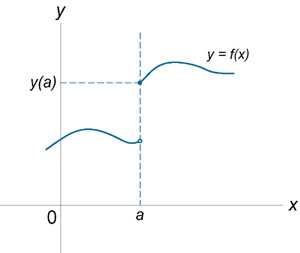
\includegraphics{img/fig1.jpg}
\caption{Discontinuity}
\end{figure}

% У заключения нет номера главы
\section*{Conclusion}
\lipsum[1-2]

\setmonofont[Mapping=tex-text]{CMU Typewriter Text}
% \bibliographystyle{plain}
% \bibliography{diploma}
\printbibliography
\end{document}
